This section provides the reader with an overview of the Turing Board. The primary operational aspects of the the Turing Board, from the perspective of end users, are defined here. The key features and functions found in the Turing Board, as well as critical user interactions and user interfaces are described in detail.

\subsection{Features \& Functions}
When desired, the Turing Board will follow the user side by side at a walking pace. When called upon, it will summon itself to the user's location from a parked spot. However, users will not be able to take advantage of the autonomous features when they mount the board. The change in inertia spawned by a computer generated movement of the longboard puts the user at great risk of losing balance when taking off, braking, and especially turning. This changes the balance of the system as a whole. Such a problem is not an issue in household autonomous vehicles such as a self-driving car because the change in inertia only affects the balance of the user and not the car in any significant way. 

The feature set of the Turing Board also consists of the collection and display of ride analytics.

Visually, the Turing Board is anticipated to share the form of any regular electric skateboard, with the only difference being that it is going to have a camera mounted on the nose end. The parts will consist of a deck, underneath the deck will comprise of an encasing that will house the battery, computation module, turning mechanism hardware, trucks and motorized wheels. The placement of the camera module is anticipated to be on the top of the board. 

On the software side, the items include a webapp hosted on an external third party server. 

\subsection{External Inputs \& Outputs}
GPS information is a critical entity that will be involved in both external input and output scenarios. We will need the account for the GPS information of both the user and the board. The user authentication is handled by the Google Firebase Authentication API paired with the Google Firebase Cloud Firestore API acting as a cloud database. 

\subsection{Product Interfaces}
Here are some of the screenshots of what the application interface will look like for the end-user. 
\begin{figure}
    \centering
    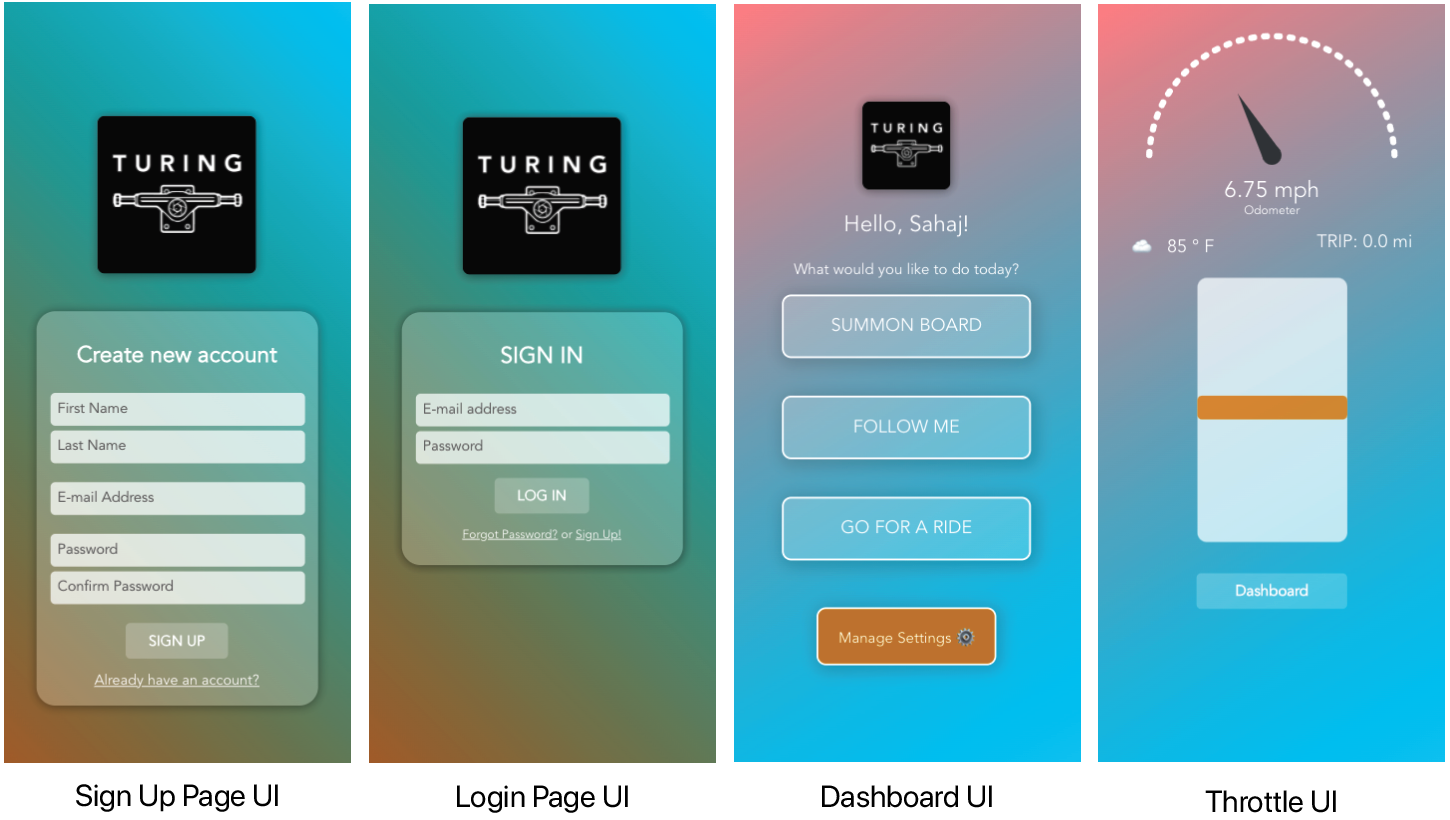
\includegraphics[width=1\textwidth]{images/UI.png} % first figure itself
    \caption{User Interface Screenshots}
\end{figure}

%Specify what all operational (visible) interfaces look like to your end-user, administrator, maintainer, etc.Show sample/mocked-up screen shots, graphics of buttons, panels, etc.  Refer to the critical externalinputs and outputs described in the paragraph above.